\chapter{Asking Texas Millionaires How They Got RICH!}

These notes follow a School of Hard Knocks interview, curated by LazyingArt LLC, but we read the conversation as something more structured than a montage of expensive cars and quick advice. The lecture begins with visible wealth, then rapidly quantifies the field in which the interviews are taking place. From there it moves through leverage, mentorship, mortality, demand shocks, reinvestment, faith, and corporate equity. The mathematics is light, but it is real: we are given a distribution, a finite-life ribbon, a scaling ratio, a small planning horizon, and finally a compact operating identity for leadership and wealth creation. Our task is to keep those formal objects tied to the order in which the lecture introduces them.

\section{Wealth Field and Entry Conditions}

We are first shown wealth as spectacle, but the lecture quickly refuses to remain on that surface. Highland Park is named as one of the wealthiest places in the United States, and the visual insert does the important work: it gives a distribution behind the claim. So before we ask how any particular individual became rich, we are told something about the environment itself.

A convenient notation for the opening chart is
\begin{align}
I &\in \{10,20,30,40,50,60,75,100,125,150,200,>200\},\\
H(I) &= \text{household count in income bin } I.
\end{align}
The smaller bins are not fully legible, so the set of bins should be read as a cautious reconstruction. What is not in doubt is the overall shape: the right tail is heavy, and the largest visible mass sits in the terminal bin.

The lecture's introductory numerical claim can be written simply as
\begin{equation}
\text{Highland Park rank}=6.
\end{equation}
This is not deep mathematics, but it matters rhetorically. The lecture is telling us that we are not sampling randomly. We are entering a field in which wealth is unusually concentrated, and therefore the next questions can be asked more sharply.

\begin{figure}[h]
\centering

\includegraphics[width=0.86\textwidth]{lecture_88_figure_02.png}
\caption{Highland Park introduction with overlaid household-income distribution. The screenshot remains important because it ties the spoken claim about local wealth directly to the visible quantitative insert.}
\end{figure}

The screenshot is worth keeping because the lecture does two things at once here. It preserves the interview setting---the street, the cars, the theater frontage---and it overlays a chart that interprets that setting numerically. The visual evidence and the spoken setup belong together.

For note writing, however, we also want a cleaner schematic of the histogram itself. The following redraw keeps only the visible structure and labels; it does \emph{not} claim exact counts.

\begin{figure}[h]
\centering
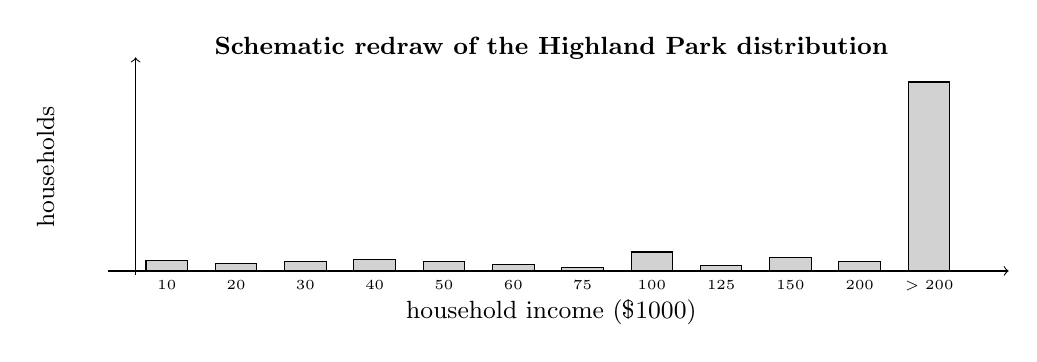
\begin{tikzpicture}[x=0.88cm,y=0.12cm]
\draw[->] (-0.4,0) -- (12.6,0);
\draw[->] (0,-0.4) -- (0,22.6);

\draw[fill=gray!35] (0.15,0) rectangle (0.75,1.1);
\draw[fill=gray!35] (1.15,0) rectangle (1.75,0.8);
\draw[fill=gray!35] (2.15,0) rectangle (2.75,1.0);
\draw[fill=gray!35] (3.15,0) rectangle (3.75,1.2);
\draw[fill=gray!35] (4.15,0) rectangle (4.75,1.0);
\draw[fill=gray!35] (5.15,0) rectangle (5.75,0.7);
\draw[fill=gray!35] (6.15,0) rectangle (6.75,0.4);
\draw[fill=gray!35] (7.15,0) rectangle (7.75,2.0);
\draw[fill=gray!35] (8.15,0) rectangle (8.75,0.6);
\draw[fill=gray!35] (9.15,0) rectangle (9.75,1.4);
\draw[fill=gray!35] (10.15,0) rectangle (10.75,1.0);
\draw[fill=gray!35] (11.15,0) rectangle (11.75,20.0);

\node[below] at (0.45,0) {\tiny 10};
\node[below] at (1.45,0) {\tiny 20};
\node[below] at (2.45,0) {\tiny 30};
\node[below] at (3.45,0) {\tiny 40};
\node[below] at (4.45,0) {\tiny 50};
\node[below] at (5.45,0) {\tiny 60};
\node[below] at (6.45,0) {\tiny 75};
\node[below] at (7.45,0) {\tiny 100};
\node[below] at (8.45,0) {\tiny 125};
\node[below] at (9.45,0) {\tiny 150};
\node[below] at (10.45,0) {\tiny 200};
\node[below] at (11.45,0) {\tiny $>200$};

\node[below] at (6,-2.0) {\small household income (\$1000)};
\node[rotate=90] at (-1.3,11) {\small households};
\node at (6,23.6) {\small \textbf{Schematic redraw of the Highland Park distribution}};
\end{tikzpicture}
\caption{Approximate redraw of the histogram structure visible in the opening insert. The dominant feature is the very large terminal $>200$ bin.}
\end{figure}

So the opening move of the lecture is already methodological. We do not merely ask, ``Who owns the expensive car?'' We first identify the statistical neighborhood in which such ownership sits.

\section{Finance, Leverage, and the First Million}

Once the field is established, the lecture moves into a repeated interview template: what do you do, how much have you made, what happened in the year of peak earnings, and were you ever broke? The first cluster of answers makes two claims simultaneously. First, there are industries and roles with direct access to very large compensation. Second, the lecture does not want us to confuse raw earnings with the mechanism that produced them.

The first executive answer is blunt: the money is in the money business. Finance, senior corporate responsibility, and proximity to large systems can produce extreme annual income. The transcript then gives a hard number:
\begin{equation}
M_{\max}=\$16.7\,\text{million}.
\end{equation}
We are also told that this speaker had been the CEO of 7-Eleven and chairman and CEO of Blockbuster. The effect is immediate. Before the lecture generalizes, it first establishes that the speaker has operated at a scale large enough to make the advice nontrivial.

But the lecture does not remain content with biography. It quickly asks what principle can be transported from one life into another. The first answer is leverage:
\begin{equation}
\text{hiring} \rightarrow \text{leverage} \rightarrow \text{scale}.
\end{equation}
This is one of the cleanest causal chains in the lecture. The point is that isolation does not scale well. A person working only through his own understanding and his own hours is bounded by that narrow pipe. Hiring broadens the pipe.

\subsection{Question \& Answer}

\paragraph{Question.} Is there a shortcut to real dreams?

\paragraph{Answer.} The lecture's answer is not that effort can be skipped. It is that error can be compressed. Mentorship is presented as a path-shortening device because it reduces avoidable mistakes and gives a straighter route through the search space.

We can write the lecture's idea schematically as
\begin{equation}
\text{mentorship} \rightarrow \text{fewer mistakes} \rightarrow \text{shorter path}.
\end{equation}
The transcript is somewhat garbled in this passage, but the structural point is clear. There is no magical bypass. There is, however, a way to waste less time.

This matters because the lecture is quietly changing levels. It begins with money, but it is already turning toward mechanism. The question is no longer merely how much was made; it is what reduces error, what creates scale, and what causes growth to accelerate rather than remain linear.

\section{Broke, Poverty, and the Ribbon of Time}

The lecture then makes a sharp conceptual distinction that prevents the chapter from collapsing into a list of income anecdotes.

\begin{definition}
In the local vocabulary of the lecture, being \emph{broke} is a reversible financial state, while \emph{poverty} names a disabling mindset.
\end{definition}

This is a useful distinction because it separates cash position from self-conception. One can be temporarily broken financially and still remain oriented toward action. One can also have more money and yet still carry the habits of paralysis.

At this point the lecture makes its strongest formal move. The speaker says, in effect, let us stop speaking vaguely and put life on a strip from \(1\) to \(100\). Average female life is marked at \(81\), average male life at \(75\), and the speaker's own age at \(57\). We can encode the ribbon data as
\begin{align}
A_f &= 81, & A_m &= 75, & a &= 57.
\end{align}
If we use the male marker as the first comparison point, then the nominal remainder is
\begin{equation}
R_{\text{nominal}} = A_m - a = 75 - 57 = 18.
\end{equation}
That is already a powerful compression. Much of the lecture up to this point has been about money, but now time becomes the scarce variable.

The lecture then immediately weakens even this simple remainder. A nominal eighteen years is not the same thing as eighteen years of equal quality. Illness, fatigue, and bodily limits eat into the supposedly available future. A cautious reconstruction of the spoken logic is
\begin{equation}
R_{\text{effective}} \le R_{\text{nominal}}.
\end{equation}
This last formula is not a line spoken as algebra, but it is exactly the structure of the argument. We are not merely counting years. We are discounting the naive remainder by the possibility that not all future years are equally usable.

\begin{figure}[h]
\centering
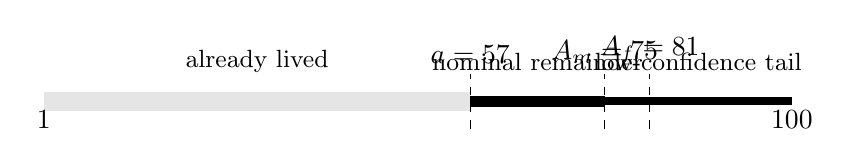
\begin{tikzpicture}[x=0.095cm,y=1cm]
\draw[line width=3pt] (0,0) -- (100,0);
\fill[gray!20] (0,-0.12) rectangle (57,0.12);
\draw[line width=4pt] (57,0) -- (75,0);
\draw[line width=1.2pt,densely dashed] (75,0) -- (100,0);

\draw[dashed] (57,-0.35) -- (57,0.35);
\draw[dashed] (75,-0.35) -- (75,0.35);
\draw[dashed] (81,-0.35) -- (81,0.35);

\node[above] at (57,0.35) {$a=57$};
\node[above] at (75,0.35) {$A_m=75$};
\node[above] at (81,0.35) {$A_f=81$};

\node[below] at (0,0) {$1$};
\node[below] at (100,0) {$100$};

\node at (28.5,0.5) {\small already lived};
\node at (66,0.5) {\small nominal remainder};
\node at (87.5,0.5) {\small low-confidence tail};
\end{tikzpicture}
\caption{Transcript-based reconstruction of the ribbon demonstration. The dashed tail represents the lecture's insistence that nominal years and usable years are not the same thing.}
\end{figure}

This is where the lecture's tempo changes. We begin with money, but the ribbon forces a more severe question: what is the real scarce good? The answer is not simply dollars. It is a finite and quality-sensitive stock of life.

\section{Opportunity Shock and the Scale Jump}

Having compressed life itself, the lecture returns to business with greater seriousness. The next case is no longer just a success story. It is a model of how an external shock can be converted into revenue by someone positioned to receive the flow.

The key numbers are
\begin{align}
M_{\text{prior}} &\approx \$1.5\,\text{million},\\
M_{\max} &= \$16.7\,\text{million},\\
N_{\text{AA}} &\approx 13{,}000.
\end{align}
Here \(M_{\text{prior}}\) is the highest annual figure before the shock, \(M_{\max}\) is the windfall year, and \(N_{\text{AA}}\) is the local employee population said to be affected by the bankruptcy event.

\paragraph{Worked example.} The lecture's logic in the hearing-aid case can be written as a short derivation.
\begin{enumerate}
\item American Airlines files bankruptcy.
\item Employees fear the possible loss of generous hearing-related benefits.
\item A large number of workers pull future usage into the present.
\item Local demand for hearing services spikes sharply.
\item Revenue jumps from \(M_{\text{prior}}\) to \(M_{\max}\).
\end{enumerate}

The scaling factor is then
\begin{equation}
\frac{M_{\max}}{M_{\text{prior}}}
\approx
\frac{16.7}{1.5}
\approx
11.1.
\end{equation}
So the lecture is not describing a modest improvement. It is describing roughly an order-of-magnitude jump.

The causal chain can be summarized as
\begin{equation}
\text{bankruptcy shock} \rightarrow \text{benefit-usage surge} \rightarrow \text{revenue jump}.
\end{equation}
This is the clearest business case study in the lecture. It is not presented as a theorem. It is presented as a mechanism: when institutions wobble, behavior changes, and a prepared business can absorb the altered flow.

The lecture then widens the lesson. Many owners make a little money and immediately become defensive. They are afraid to lose what they finally earned, and so they begin to clutch rather than compound. The answer given here is aggressive reinvestment: do not let the first taste of success turn into fear. In the logic of the lecture, fear freezes scale, while reinvestment maintains it.

\section{Faith, Discipline, and the One--Three--Five Horizon}

After the demand-shock case, the lecture makes another pivot. It becomes explicit that wealth creation is not being treated as purely technical. Faith enters not as decoration, but as stabilizer. The claim is that without something larger than the self, the business owner has no durable support when conditions stop being favorable.

That argument should not be flattened into a generic moralism. In the transcript it follows a very practical business discussion. Its function is to answer a real question: what keeps a person from disintegrating when the environment turns hard? The lecture's answer is spiritual grounding and gratitude.

The next interview returns to more visible symbols of success---a G-Wagon, a later family life, discretionary spending---but again the lecture moves behind the symbol. Wasteful status consumption is treated as an error of timing. Clubs, bottle service, and spectacle absorb money and attention before compounding has done its work. This is paired with an older person's claim that quality of time matters more than mere quantity. In that sense the G-Wagon advice quietly echoes the ribbon demonstration: the scarce resource is not only money, but the way one uses limited life.

The explicit planning device here is the one--three--five horizon:
\begin{equation}
G=\{1,3,5\}.
\end{equation}
The lecture does not formalize this further, but it is natural to read the set as an ordered ladder of near, medium, and longer horizons:
\begin{itemize}
\item \(1\): a near target that proves motion,
\item \(3\): a medium horizon on which habits begin to compound,
\item \(5\): a sufficiently distant goal to organize ambition without dissolving into fantasy.
\end{itemize}
The important thing is not the numerology. It is the structure. Goals are staged, and each completed stage feeds motivation into the next.

So by the end of this section, the lecture has brought together three strands that often get kept apart: faith under adversity, discipline against premature spectacle, and a small but ordered horizon of goals.

\section{CEO Logic: Change, Confidence, Clarity}

The final interview is the most compressed and therefore, in some sense, the most mathematical. The speaker offers a triad: change, confidence, clarity. The transcript stumbles briefly around the second item, but the intended structure is plain enough.

The first slogan is the lecture's cleanest identity:
\begin{equation}
\text{change}=\text{opportunity}.
\end{equation}
Of course this is not an algebraic equality. It is a leadership rule. The lecture means that change becomes opportunity for the agent who can read it, absorb it, and act while others resist it.

\subsection{Question \& Answer}

\paragraph{Question.} How does change become opportunity?

\paragraph{Answer.} Not automatically. The lecture's answer is comparative. When change arrives, most people experience it first as disturbance. If we respond well while others hesitate, the same event becomes a source of value. The opportunity is not in the mere existence of change; it is in relative response.

The next relation, stated here as a cleaned reconstruction of the speaker's point, is
\begin{equation}
\text{confidence}\propto \text{preparation}.
\end{equation}
This is not a board equation, but it faithfully expresses the logic of the passage. Confidence is not supposed to be mood. It is supposed to be the effect of preparation. The more preparation, the more warranted confidence.

The third term is clarity. Simplicity is treated here as an achievement rather than as a reduction. To keep things simple when they are actually complex is a leadership skill. Communication matters because strategy does not travel unless other people can understand it.

\begin{figure}[h]
\centering
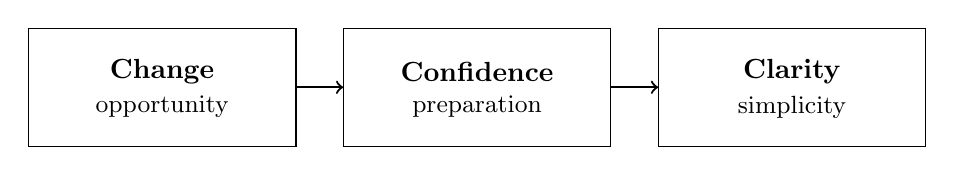
\begin{tikzpicture}
\draw (0,0) rectangle (3.4,1.5);
\draw (4,0) rectangle (7.4,1.5);
\draw (8,0) rectangle (11.4,1.5);

\node at (1.7,0.95) {\textbf{Change}};
\node at (1.7,0.50) {\small opportunity};

\node at (5.7,0.95) {\textbf{Confidence}};
\node at (5.7,0.50) {\small preparation};

\node at (9.7,0.95) {\textbf{Clarity}};
\node at (9.7,0.50) {\small simplicity};

\draw[->,thick] (3.4,0.75) -- (4,0.75);
\draw[->,thick] (7.4,0.75) -- (8,0.75);
\end{tikzpicture}
\caption{Transcript-backed reconstruction of the closing framework. The lecture compresses leadership into three linked moves: accept change, prepare enough to respond with confidence, and communicate with clarity.}
\end{figure}

The lecture then closes its corporate argument with a distinction between salary and ownership. Let
\begin{align}
S &= \text{salary},\\
E &= \text{equity}.
\end{align}
The lesson is not that salary is useless. Salary pays bills, keeps a life running, and can stabilize a career. But the lecture insists that the real creation of wealth in the corporate world comes through ownership:
\begin{equation}
\text{wealth}_{\text{corporate}} \approx \text{equity accumulation}.
\end{equation}
The example of the former administrative assistant at SpaceX is introduced precisely to make this point. If a worker can buy into equity, then future repricing matters more than current paycheck size. This is why the lecture treats salary and wealth as different categories. The paycheck sustains the present; equity carries exposure to the future.

We can therefore summarize the closing mechanism as follows:
\begin{equation}
\text{prepared response} \rightarrow \text{shareholder value}.
\end{equation}
This is where the lecture ends most strongly. It does not end with the luxury object. It ends with a compact operating theory: welcome change, prepare enough to stand inside it, simplify enough to lead through it, and own enough equity that value creation can stick.

\section{Summary}

The lecture begins with the sight of wealth, but it does not remain trapped there. It quantifies the field through the Highland Park distribution, turns immediately to leverage and mentorship, and then makes a surprisingly sharp move into a finite-life model built on a ribbon from \(1\) to \(100\). From there it returns to business through a concrete demand shock, extracts a scaling ratio, folds in faith and disciplined goal horizons, and closes with the CEO triad of change, confidence, and clarity.

What survives the lecture best is not a single slogan, though the lecture produces several. It is a sequence of formal reductions. Wealth field before wealth anecdote. Leverage before effort alone. Time scarcity before money vanity. Shock converted into flow. Salary distinguished from equity. In that sense the chapter is disciplined by the same principle the lecture ends with: keep the structure clear enough that the mechanism can be seen.